
To communicate with a computer, one is required to 'speak' the same language as the computer. A computer's language is pre-defined by the producer of the computer, and generally referred to as \emph{machine code} or \emph{machine instructions}.\\
Today's software developers make use of various programming languages and each language deals with an area of functionality. These languages have to be translated for the computer and this is done with tools called compilers.\\
When developing, the choice of programming language can be vital to the project's success and functionality.\\\\
In this report, a description of the development-process of a new language is laid out.

\section{\langname{}}
In this project it is wanted to address the interest for a role-playing based language. The purpose of the language is to define characters, skills, attributes, effects etc, commonly found in \ac{rpgs}.

To do this a language is constructed, which should catch the intuitive and simple characteristics of character sheets. Character sheets can be thought of as information containers for various \ac{rpgs}. They keep track of the character's skill- and health-state as well as inventory (for reference see appendix \vref{charsheet}).

\section{Role-playing}
\ac{rpgs} have been commercially available since the 1970's and exist in various forms. \ac{rpgs} can be described as interactive storytelling, meaning that the players take part in ''writing'' the adventure being played. When actions are unrestricted and players are free to do as they please the adventure becomes more than a story, evolving into an interactive activity between the players and the storyteller.
There are currently three types available; \emph{Computer-}, \emph{\ac{pnp}-} and \emph{Live Action \ac{rpgs}}, the first two being a focus in this project.

In \ac{rpgs}, players take on the roles of fictitious characters, most often created by the players themselves.

When playing \emph{\ac{pnp}- \ac{rpgs}}, a core rulebook is used, to solve conflicts, get inspiration for adventures, character creation, reference and more. In \emph{Computer- \ac{rpgs}}, the rulebook is replaced with static rules implemented in the game world, however developers often provide useful information (much like rulebooks) for the players in the form of a guide or a codex.
Characters are defined by their abilities and attributes, meaning that each ability is assigned a number that represents how 'good' the character is using a given ability. This is also the case with attributes and certain 'traits' (e.g superpowers and disciplines). An attribute is value on a scale of some minimum number to some maximum, where each value indicates how much better or worse a character is compared to other beings in the game world. Take for example the attributes strength and charisma. Strength tells you how strong a character is, often used to measure how much they can lift and how hard they can hit. Charisma is a character's social skill level, used to measure how well they can handle social situations. Most games break as much as possible down to numbers; appearance, intellect, luck and more.
This should in a way contribute to the level of realism in events and outcomes while playing.

The first modern \emph{\ac{pnp} \ac{rpg}} to be released commercially is the game \emph{\ac{dnd}}, which was first published in 1974.\cite{wikidnd}
\emph{\ac{dnd}} can therefore be thought of as the pioneer of role-playing games.

\subsection{Character creation}

How a character is created varies from system to system. Common for most is that the characters all have statistics (stats) describing them.
Stats are the term used for all numerical values in the character description. They can indicate a certain status amongst peers (e.g on a scale of 0 - 10), serve as a counter for how often a certain ability or item can be used, tell a character's level of skill and/or trait (such as Strength) and last but not least they keep track of the character's resources (such as \ac{hp}).
\ac{hp} is a measure for how much damage a character can take before dying. Strength can be used to calculate how much damage a character can do to others. Depending on what stat is in question, it can be decided by rolling dice, be computed from other stats, assigned specifically by the player or based on the player's choice of race.

\subsection{Pen \& Paper}
\todo{More details about GM}
When playing \emph{\ac{pnp}} the players generally use various dice (see figure \ref{dice}) to determine an outcome of an activity, for example an attack, where the outcome determines if the attack is successful and thereafter how much damage is inflicted. To help keep track of a character's attributes and other information, a character sheet is used.

In \ac{pnp} games the participants are: A \ac{gm}, who is responsible for control of non-player characters, environment, the setting of the adventure and has the final say in conflicts. The players control their individual characters, around which the adventure revolves.

A game scenario can be described as following: The \ac{gm} prepares an adventure for the players and lays down additional rules if needed. Participants are seated around a table with their character sheets and a number of dice. Each player has created a character to use in the given adventure. The \ac{gm} describes the setting and series of events, playing all non-player characters. The players roleplay their characters and determine their actions by themselves. When an action is required from a specific player, they can determine the outcome of the action by rolling a specific set of dice.
\begin{figure}[!h]
\centering
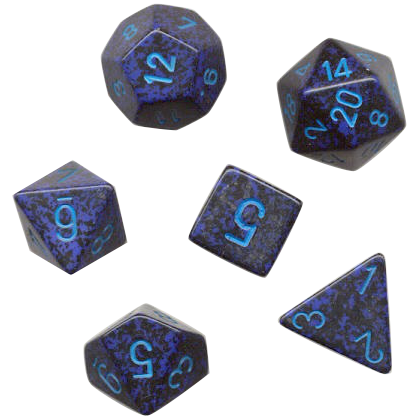
\includegraphics[scale=0.35]{img/rpgdice.png}
\caption{Dice for role-playing purposes}
%\cite{rpgdice}
\label{dice}
\end{figure}

\subsection{Digitised}
In \emph{Computer \ac{rpgs}} the outcome of an activity is determined by measures implemented by the developers. This can be an imitation of a dice roll (variation) or a static calculation (pre-calculated).
To keep track of character information, a digitised character sheet is often accessible, where the player can customise their character to some degree.\\
In computer \ac{rpgs} the player will often be given a set of possible actions to choose from, and it is up to the player to determine which one suits the situation best. The opponents are pre-programmed to react in a certain way to various events, such as low \ac{hp}.

\pagebreak

%source: (wikidnd) http://en.wikipedia.org/wiki/History_of_role-playing_games